\documentclass[twocolumn,aps,prapplied,superscriptaddress,floatfix]{revtex4-2}

\usepackage{amsmath}
\usepackage{amssymb}
\usepackage{graphicx}
\usepackage{xcolor}
\usepackage{booktabs}
\usepackage[hidelinks]{hyperref}

% Auto-generated by generate_unified_assets.py -- DO NOT EDIT BY HAND.
\newcommand{\NumBackends}{3}
\newcommand{\ChipQubits}{156}
\newcommand{\NumCampaigns}{7}
\newcommand{\NumZenodoLetters}{6}
\newcommand{\NumZenodoPreregs}{5}
\newcommand{\TotalJobs}{42}
\newcommand{\TotalPubs}{1{,}062}
\newcommand{\ShotsPerPub}{2{,}048}
\newcommand{\TotalShots}{2{,}174{,}976}
\newcommand{\TotalQpuSeconds}{673}
\newcommand{\MarrakeshJobs}{16}
\newcommand{\MarrakeshPubs}{630}
\newcommand{\MarrakeshShots}{1{,}290{,}240}
\newcommand{\MarrakeshSeconds}{392}
\newcommand{\FezJobs}{13}
\newcommand{\FezPubs}{216}
\newcommand{\FezShots}{442{,}368}
\newcommand{\FezSeconds}{139}
\newcommand{\KingstonJobs}{13}
\newcommand{\KingstonPubs}{216}
\newcommand{\KingstonShots}{442{,}368}
\newcommand{\KingstonSeconds}{142}
\newcommand{\TmapSeriesJobs}{14}
\newcommand{\TmapSeriesShots}{1{,}159{,}168}
\newcommand{\TmapSeriesSeconds}{341}
\newcommand{\RoSeriesJobs}{27}
\newcommand{\RoSeriesShots}{516{,}096}
\newcommand{\RoSeriesSeconds}{193}
\newcommand{\CnJobs}{1}
\newcommand{\CnPubs}{244}
\newcommand{\CnShots}{499{,}712}
\newcommand{\CnCouplerShots}{4{,}997{,}120}
\newcommand{\CnSeconds}{139}
\newcommand{\DoiCnZeroOne}{10.5281/zenodo.24406435}
\newcommand{\DoiTmapTwo}{10.5281/zenodo.24406426}
\newcommand{\DoiTmapThree}{10.5281/zenodo.24406525}
\newcommand{\DoiTmapThreePrereg}{10.5281/zenodo.24406496}
\newcommand{\DoiTmapFour}{10.5281/zenodo.24407001}
\newcommand{\DoiTmapFourPrereg}{10.5281/zenodo.24406640}
\newcommand{\DoiTmapFive}{10.5281/zenodo.24407875}
\newcommand{\DoiTmapFivePrereg}{10.5281/zenodo.24407538}
\newcommand{\DoiRoSixSeven}{10.5281/zenodo.24420902}
\newcommand{\DoiRoSixPrereg}{10.5281/zenodo.24407897}
\newcommand{\DoiRoSevenPrereg}{10.5281/zenodo.24419327}
\newcommand{\CapsuleRfcShaPrefix}{9631f34a6c54d7eb}
\newcommand{\CapsuleSourceCount}{125}
\newcommand{\CampaignRegistryRows}{TMAP-02 & 2026-11-16 & \texttt{marrakesh} & 1 & 90 & 184{,}320 & 53 & -- & 24406426\\
CN-01 & 2026-11-16 & \texttt{marrakesh} & 1 & 244 & 499{,}712 & 139 & -- & 24406435\\
TMAP-03 & 2026-11-20 & \texttt{marrakesh} & 1 & 80 & 163{,}840 & 47 & 24406496 & 24406525\\
TMAP-04 & 2026-11-20 & All 3 QPUs & 6 & 198 & 405{,}504 & 121 & 24406640 & 24407001\\
TMAP-05 & 2026-11-20 & All 3 QPUs & 6 & 198 & 405{,}504 & 120 & 24407538 & 24407875\\
RO-06 & 2026-11-20..21 & All 3 QPUs & 24 & 144 & 294{,}912 & 128 & 24407897 & 24420902\\
RO-07 & 2026-11-21 & All 3 QPUs & 3 & 108 & 221{,}184 & 65 & 24419327 & 24420902\\
\hline
\textbf{Total} & Nov 16--21 & 3 Heron r2 & \textbf{42} & \textbf{1{,}062} & \textbf{2{,}174{,}976} & \textbf{673} & 5 DOIs & 6 DOIs\\}
\newcommand{\TmapCircuitQubits}{40}
\newcommand{\TmapChainCz}{39}
\newcommand{\TmapChainDepth}{66}
\newcommand{\TmapStarOptThreeCz}{79}
\newcommand{\TmapStarOptOneCz}{147}
\newcommand{\TmapStarFreeCz}{163}
\newcommand{\TmapSeedThetaDeg}{51.7}
\newcommand{\TmapBlocks}{10}
\newcommand{\TmapBlocksDf}{9}
\newcommand{\TmapCandidatePaths}{400}
\newcommand{\TmapWilcoxonFloorP}{0.010}
\newcommand{\TmapTwoJobId}{dbto408n26qs739tnrj0}
\newcommand{\TmapTwoPubs}{90}
\newcommand{\TmapTwoShots}{184{,}320}
\newcommand{\TmapTwoSeconds}{53}
\newcommand{\TmapTwoUnionQubits}{96}
\newcommand{\TmapTwoUnionRoPct}{2.47}
\newcommand{\TmapTwoRewriteOptThreePp}{+14.27}
\newcommand{\TmapTwoRewriteOptOnePp}{+12.47}
\newcommand{\TmapTwoPathGapPp}{+10.54}
\newcommand{\TmapTwoPathGapCi}{[+9.95, +11.12]}
\newcommand{\TmapTwoBestFcl}{0.215}
\newcommand{\TmapTwoMedFcl}{0.110}
\newcommand{\TmapTwoStockFcl}{0.158}
\newcommand{\TmapTwoStarFreeFcl}{0.016}
\newcommand{\TmapTwoVsStockPp}{+5.70}
\newcommand{\TmapTwoAaVirtualZPp}{-0.24}
\newcommand{\TmapTwoAaVirtualZCi}{[-0.88, +0.41]}
\newcommand{\TmapTwoAaVirtualZP}{0.43}
\newcommand{\TmapTwoMaxHolmP}{$6.6\times10^{-9}$}
\newcommand{\TmapStarHubDeg}{20}
\newcommand{\TmapTwoQFortyTwoPct}{22.3}
\newcommand{\TmapTwoQFortyOnePct}{12.1}
\newcommand{\TmapTwoQThirtyOnePct}{12.2}
\newcommand{\TmapTwoQFortySixPct}{1.3}
\newcommand{\TmapTwoQFortyTwoIbmPct}{1.0}
\newcommand{\TmapTwoQFortyOneIbmPct}{1.3}
\newcommand{\TmapProbeSecLow}{5}
\newcommand{\TmapProbeSecHigh}{6}
\newcommand{\TmapThreeDaysLater}{4}
\newcommand{\TmapThreeJobId}{dc0ajv5s2omc738915k0}
\newcommand{\TmapThreePubs}{80}
\newcommand{\TmapThreeShots}{163{,}840}
\newcommand{\TmapThreeSeconds}{47}
\newcommand{\TmapThreeUnionQubits}{81}
\newcommand{\TmapThreePathGapPp}{-4.29}
\newcommand{\TmapThreePathGapCi}{[-5.24, -3.33]}
\newcommand{\TmapThreePathGapP}{$6.4\times10^{-6}$}
\newcommand{\TmapThreeBestFcl}{0.101}
\newcommand{\TmapThreeMedFcl}{0.144}
\newcommand{\TmapThreeBestMitFcl}{0.651}
\newcommand{\TmapThreeMedMitFcl}{0.481}
\newcommand{\TmapThreeMitGapPp}{+17.03}
\newcommand{\TmapThreeReadoutShiftPp}{+21.3}
\newcommand{\TmapThreeReadoutShiftP}{$1.8\times10^{-6}$}
\newcommand{\TmapThreeInteractionPp}{-5.64}
\newcommand{\TmapThreeInteractionP}{$1.0\times10^{-6}$}
\newcommand{\TmapThreeStarGapPp}{+1.35}
\newcommand{\TmapThreeStockReplayGapPp}{-5.26}
\newcommand{\TmapThreeStockTodayGapPp}{-1.75}
\newcommand{\TmapThreeQFortySixMeanPct}{35.0}
\newcommand{\TmapThreeQFortySixZeroToOnePct}{54.4}
\newcommand{\TmapThreeQFortySixOneToZeroPct}{15.5}
\newcommand{\TmapThreeQThirtyOneOneToZeroPct}{44.8}
\newcommand{\TmapThreeQFortySixIbmPct}{1.1}
\newcommand{\TmapTwoLockShaPrefix}{5f4a04c45933e046}
\newcommand{\TmapThreeLockShaPrefix}{ea7e8765a9d82f4c}
\newcommand{\TmapFourTotalSeconds}{121}
\newcommand{\TmapFiveTotalSeconds}{120}
\newcommand{\TmapProbePubs}{6}
\newcommand{\TmapMainPubs}{60}
\newcommand{\TmapExclThresholdPct}{15}
\newcommand{\TmapFourHelpsCount}{1}
\newcommand{\TmapFiveHelpsCount}{2}
\newcommand{\TmapDtMinLow}{82}
\newcommand{\TmapDtMinHigh}{85}
\newcommand{\TmapFourMarrLonePp}{+25.02}
\newcommand{\TmapFourMarrLoneCi}{[+24.16, +25.89]}
\newcommand{\TmapFourMarrLoneP}{$6.8\times10^{-13}$}
\newcommand{\TmapFourMarrLfourMitPp}{-10.1}
\newcommand{\TmapFiveMarrMonePp}{-0.29}
\newcommand{\TmapFiveMarrMtwoPp}{+2.71}
\newcommand{\TmapFiveMarrMfourPp}{-3.00}
\newcommand{\TmapFiveMarrMfourCi}{[-4.34, -1.67]}
\newcommand{\TmapFiveMarrMfourP}{0.002}
\newcommand{\TmapFourFezLonePp}{-3.60}
\newcommand{\TmapFourFezLoneCi}{[-4.37, -2.83]}
\newcommand{\TmapFourFezLoneP}{$4.6\times10^{-6}$}
\newcommand{\TmapFourFezLfourMitPp}{-19.6}
\newcommand{\TmapFiveFezMonePp}{+2.26}
\newcommand{\TmapFiveFezMtwoPp}{-4.64}
\newcommand{\TmapFiveFezMfourPp}{+6.90}
\newcommand{\TmapFiveFezMfourCi}{[+5.62, +8.18]}
\newcommand{\TmapFiveFezMfourP}{$1.4\times10^{-6}$}
\newcommand{\TmapFourKingLonePp}{-0.25}
\newcommand{\TmapFourKingLoneCi}{[-1.62, +1.13]}
\newcommand{\TmapFourKingLoneP}{1.00}
\newcommand{\TmapFourKingLfourMitPp}{-9.2}
\newcommand{\TmapFiveKingMonePp}{+4.65}
\newcommand{\TmapFiveKingMtwoPp}{-3.16}
\newcommand{\TmapFiveKingMfourPp}{+7.81}
\newcommand{\TmapFiveKingMfourCi}{[+6.58, +9.03]}
\newcommand{\TmapFiveKingMfourP}{$6.3\times10^{-7}$}
\newcommand{\TmapSignReversalRows}{ibm\_marrakesh & 85\,m & +25.02 [+24.16, +25.89] & -10.1 & -3.00 [-4.34, -1.67] & -0.29 & +2.71\\
ibm\_fez & 84\,m & -3.60 [-4.37, -2.83] & -19.6 & +6.90 [+5.62, +8.18] & +2.26 & -4.64\\
ibm\_kingston & 82\,m & -0.25 [-1.62, +1.13] & -9.2 & +7.81 [+6.58, +9.03] & +4.65 & -3.16\\}
\newcommand{\TmapFourMarrProbeFcl}{0.313}
\newcommand{\TmapFourMarrCalFcl}{0.063}
\newcommand{\TmapFourQFortySixPct}{34.4}
\newcommand{\TmapFiveQFortySixPct}{0.6}
\newcommand{\TmapFourMarrUtc}{20:26}
\newcommand{\TmapFiveMarrUtc}{21:51}
\newcommand{\TmapFourKingQOneZeroSevenPct}{19.8}
\newcommand{\TmapFourKingQOneZeroSevenIbmPct}{1.0}
\newcommand{\TmapFiveFezQElevenPct}{22.8}
\newcommand{\TmapFiveKingQOneZeroSevenPct}{19.1}
\newcommand{\RoSixJobs}{24}
\newcommand{\RoSevenJobsCount}{3}
\newcommand{\RoSixRounds}{8}
\newcommand{\RoSixIntervalMin}{15}
\newcommand{\RoFaultThreshPct}{15}
\newcommand{\RoIbmOkThreshPct}{3}
\newcommand{\RoRecoveredThreshPct}{5}
\newcommand{\RoContextThreshPp}{5.0}
\newcommand{\RoOvernightGapHours}{13.7}
\newcommand{\RoActiveSpanHours}{1.63}
\newcommand{\RoKingstonUnchangedHours}{16.0}
\newcommand{\RoEverHidden}{6}
\newcommand{\RoRecoveredCount}{6}
\newcommand{\RoPersistFaultPct}{87.4}
\newcommand{\RoPersistOkPct}{0.63}
\newcommand{\RoFisherOr}{1{,}095}
\newcommand{\RoFisherP}{$1.7\times10^{-122}$}
\newcommand{\RoSensPersistFaultPct}{88.0}
\newcommand{\RoSensPersistOkPct}{0.51}
\newcommand{\RoSensFisherOr}{1{,}424}
\newcommand{\RoSensFisherP}{$5.4\times10^{-109}$}
\newcommand{\RoWithinSpreadPp}{0.59}
\newcommand{\RoBetweenChangePp}{1.67}
\newcommand{\RoFezOldRho}{0.813}
\newcommand{\RoFezOldGapPp}{0.21}
\newcommand{\RoFezNewRhoRoundSix}{0.953}
\newcommand{\RoFezNewRhoRoundSeven}{0.952}
\newcommand{\RoFezNewGapRoundSevenPp}{0.12}
\newcommand{\RoTransitionOkOk}{3{,}169}
\newcommand{\RoTransitionOkFault}{20}
\newcommand{\RoTransitionFaultOk}{11}
\newcommand{\RoTransitionFaultFault}{76}
\newcommand{\RoRhoMarr}{0.71}
\newcommand{\RoRhoFez}{0.83}
\newcommand{\RoRhoKing}{0.71}
\newcommand{\RoSevenRepeats}{6}
\newcommand{\RoSevenLagMin}{39}
\newcommand{\RoSevenMaxMuxPp}{1.16}
\newcommand{\RoSevenMaxNbrPp}{1.61}
\newcommand{\RoSevenMaxAbsDPp}{1.61}
\newcommand{\RoSevenControlsMaxPp}{0.33}
\newcommand{\RoSevenTestedQubits}{19}
\newcommand{\TmapFiveFezStockFcl}{0.300}
\newcommand{\AlphaFwer}{0.05}
\newcommand{\CiLevelPct}{95}
\newcommand{\ProbeRepeats}{3}
\newcommand{\RoSevenDisagreeTotal}{9}
\newcommand{\RoSevenDisagreeRecovered}{5}
\newcommand{\RoSevenMarrQOneElevenPrePct}{31.7}
\newcommand{\RoSevenMarrQOneElevenPostPct}{2.0}
\newcommand{\RoMinHiddenMean}{0.125}
\newcommand{\RoMaxHiddenMean}{0.500}
\newcommand{\RoFezUpdatedQubits}{153}
\newcommand{\RoStalenessSummaryRows}{ibm\_marrakesh & 0 0 0 0 0 0 1 3 & 0.500 & 0.71 & \texttt{155 0 0 0 0 0 0 0} & 1.16 & 1.36\\
ibm\_fez & 0 1 0 0 0 0 0 0 & 0.125 & 0.83 & \texttt{153 0 0 0 0 0 0 153} & 0.43 & 0.99\\
ibm\_kingston & 1 0 0 0 0 0 0 0 & 0.125 & 0.71 & \texttt{0 0 0 0 0 0 0 0} & 0.81 & 1.61\\}
\newcommand{\CnJobId}{dbtp67dav06s73cfbsm0}
\newcommand{\CnTotalCouplers}{10}
\newcommand{\CnTrainCouplers}{4}
\newcommand{\CnHeldOutCouplers}{6}
\newcommand{\CnHeldOutDf}{5}
\newcommand{\CnMinHops}{5}
\newcommand{\CnBlocks}{5}
\newcommand{\CnLockedConds}{23}
\newcommand{\CnAThreeConds}{19}
\newcommand{\CnBicGate}{8}
\newcommand{\CnDdWindowUs}{8.192}
\newcommand{\CnLongWindowUs}{16.384}
\newcommand{\CnDdSixteenPulses}{16}
\newcommand{\CnDdThirtyTwoPulses}{32}
\newcommand{\CnSlotNs}{512}
\newcommand{\CnMaxStaggerNs}{256}
\newcommand{\CnCollisionStepNs}{48}
\newcommand{\CnStepGate}{0.75}
\newcommand{\CnFastBoundPp}{1.0}
\newcommand{\CnAaRmsRawPp}{1.15}
\newcommand{\CnStepFractionS}{0.62}
\newcommand{\CnWhiteFloorCapKhz}{40}
\newcommand{\CnSolvedWhiteFloorKhz}{57.2}
\newcommand{\CnRamseySixteenMean}{0.723}
\newcommand{\CnEchoSixteenMean}{0.896}
\newcommand{\CnDdThirtyTwoSixteenMean}{0.917}
\newcommand{\CnLockShaPrefix}{38ebfe7f7c007633}
\newcommand{\CnQpyShaPrefix}{158de03260c429c8}
\newcommand{\CnAmendShaPrefix}{7fb094d7a3474965}
\newcommand{\CnCdfsMeanPp}{+0.43}
\newcommand{\CnCdfsCi}{[-0.13, +1.00]}
\newcommand{\CnCdfsP}{0.47}
\newcommand{\CnCspecMeanPp}{-0.20}
\newcommand{\CnCspecCi}{[-0.50, +0.11]}
\newcommand{\CnCspecP}{0.53}
\newcommand{\CnCstagMeanPp}{+0.20}
\newcommand{\CnCstagCi}{[-0.22, +0.62]}
\newcommand{\CnCstagP}{0.61}
\newcommand{\CnCmemMeanPp}{-0.14}
\newcommand{\CnCmemCi}{[-2.25, +1.97]}
\newcommand{\CnCmemP}{0.89}
\newcommand{\CnContrastRows}{$C_{\mathrm{DFS}}$ & \multicolumn{3}{l}{$\Phi^+$ vs $\Psi^+$ stagger asymmetry ($0\to256$\,ns)} & +0.43 & [-0.13, +1.00] & 0.47\\
$C_{\mathrm{spec}}$ & \multicolumn{3}{l}{Spectator in $|{+}\rangle$ minus $|0\rangle$} & -0.20 & [-0.50, +0.11] & 0.53\\
$C_{\mathrm{stag}}$ & \multicolumn{3}{l}{$\Phi^+(256\,\mathrm{ns})-\Phi^+(0\,\mathrm{ns})$} & +0.20 & [-0.22, +0.62] & 0.61\\
$C_{\mathrm{mem}}$ & \multicolumn{3}{l}{DD32 minus Hahn echo at $16.384\,\mu$s} & -0.14 & [-2.25, +1.97] & 0.89\\}
\newcommand{\CnLockedDeltaBic}{10{,}263}
\newcommand{\CnLockedBicHZero}{10{,}437}
\newcommand{\CnLockedBicHThree}{173.7}
\newcommand{\CnHoRmseHZero}{0.130}
\newcommand{\CnHoRmseHThree}{0.143}
\newcommand{\CnHoTStat}{-0.24}
\newcommand{\CnHoPVal}{0.82}
\newcommand{\CnAThreeBicHZero}{115.05}
\newcommand{\CnAThreeBicHOne}{115.27}
\newcommand{\CnAThreeRunnerUpGap}{0.22}
\newcommand{\CnModelBicRows}{Local white ($H_0$) & local & 5 & 10{,}420.9 & 10{,}436.6 & 100.3 & 115.05\\
Local $1/f$ + white ($H_{0,1/f}$) & local & 6 & -- & -- & 825.6 & 843.22\\
Local OU bath ($H_{3,\mathrm{loc}}$) & local & 7 & -- & -- & 825.4 & 845.97\\
Static spectator $ZZ$ ($H_1$) & non-local & 6 & 2{,}482.6 & 2{,}501.4 & 97.6 & 115.27\\
Correlated Markov ($H_2$) & non-local & 7 & 10{,}361.5 & 10{,}383.4 & 95.2 & 115.83\\
Correlated OU bath ($H_3$) & non-local & 8 & 148.6 & 173.7 & 825.4 & 848.92\\
Pulse collision & apparatus & 6 & 10{,}402.6 & 10{,}421.4 & 100.3 & 118.00\\}
\newcommand{\CnValTotalReps}{550}
\newcommand{\CnValLocalNullReps}{400}
\newcommand{\CnValLocalStageTwoLowPct}{95}
\newcommand{\CnValLocalStageTwoHighPct}{100}
\newcommand{\CnValOneFMedDbic}{3{,}397}
\newcommand{\CnValDetunedMedDbic}{17{,}456}
\newcommand{\CnValOuMedDbic}{415}
\newcommand{\CnValOneFHThreePct}{100}
\newcommand{\CnValAThreeLocalFpPct}{0}
\newcommand{\CnValAThreeFastPowPct}{44}
\newcommand{\CnValAThreeMarkovPowPct}{56}
\newcommand{\CnValidationRows}{Local white ($H_0$) & 100 & 0 & 0\% & 0\% & 0\% & 0\%\\
Local $1/f$ dephasing & 100 & 3{,}397 & 100\% & 100\% & 0\% & 0\%\\
Local $1/f$ + Ramsey detuning & 100 & 17{,}456 & 100\% & 99\% & 0\% & 0\%\\
Local Ornstein--Uhlenbeck & 100 & 415 & 100\% & 95\% & 0\% & 0\%\\
Spatially correlated Markov ($H_2$) & 50 & 462 & 0\% & 0\% & 56\% & 56\%\\
Correlated OU bath, fast ($H_3$) & 50 & 1{,}289 & 100\% & 100\% & 44\% & 44\%\\
Correlated OU bath, slow ($H_3$) & 50 & 582 & 100\% & 96\% & 0\% & 0\%\\}


\begin{document}

\title{Calibration Staleness, Transient Readout Telegraphing, and Colored-Noise False Positives Across Three 156-Qubit Superconducting Quantum Processors}

\author{Devin Phillip Davis}
\affiliation{Agile Defense Systems LLC}

\date{November 22, 2026}

\begin{abstract}
Benchmarking layout compilation, error mitigation, and bath-correlation hypotheses on utility-scale superconducting quantum processors routinely relies on two implicit stationarity assumptions: that provider-published device calibration snapshots accurately rank physical qubits during job execution, and that independent Markovian (white-noise) models form an adequate statistical null for diagnosing non-local or non-Markovian error channels. Here we synthesize \NumCampaigns{} preregistered hardware campaigns (\TotalJobs{} IBM Quantum jobs, \TotalPubs{} primitive unified blocs at \ShotsPerPub{} shots each, \TotalShots{} physical circuit shots, and \TotalQpuSeconds{}\,s of charged QPU execution) across all \NumBackends{} \ChipQubits{}-qubit Heron~r2 heavy-hex processors (\texttt{ibm\_marrakesh}, \texttt{ibm\_fez}, and \texttt{ibm\_kingston}). First, in \TmapCircuitQubits{}-qubit compilation benchmarks at a fixed \TmapChainCz{}-CZ gate count and depth~\TmapChainDepth{} (\texttt{TMAP-02}--\texttt{TMAP-05}, \TmapSeriesJobs{} jobs, \TmapSeriesShots{} shots), moving from a calibration-ranked best path to a median path initially shifted classical fidelity $F_{\mathrm{cl}}$ by \TmapTwoPathGapPp\,pp, yet replaying the identical physical qubits \TmapThreeDaysLater{} days later reversed the contrast to \TmapThreePathGapPp\,pp ($p_{\mathrm{Holm}}=\TmapThreePathGapP$) due to an unflagged readout fault on \texttt{q46} (\TmapThreeQFortySixMeanPct\% measured assignment error vs \TmapThreeQFortySixIbmPct\% published). Testing a pre-job all-qubit readout probe across all \NumBackends{} processors and repeating the identical protocol \TmapDtMinLow{}--\TmapDtMinHigh{} minutes later flipped the sign of the probe-versus-calibration contrast on every processor (\TmapFourMarrLonePp$\to$\TmapFiveMarrMfourPp\,pp on \texttt{ibm\_marrakesh}, \TmapFourFezLonePp$\to$\TmapFiveFezMfourPp\,pp on \texttt{ibm\_fez}, and \TmapFourKingLonePp$\to$\TmapFiveKingMfourPp\,pp on \texttt{ibm\_kingston}), while tensored readout mitigation restored calibration-path superiority on all \NumBackends{} devices (\TmapFourMarrLfourMitPp, \TmapFourFezLfourMitPp, and \TmapFourKingLfourMitPp\,pp). Second, full-chip longitudinal readout monitoring and context-isolation experiments (\texttt{RO-06} and \texttt{RO-07}, \RoSeriesJobs{} jobs, \RoSeriesShots{} shots) show that hidden faults ($>\RoFaultThreshPct\%$ actual vs $<\RoIbmOkThreshPct\%$ listed) are transient (\RoRecoveredCount{} of \RoEverHidden{} recovered below \RoRecoveredThreshPct\%), persist across \RoSixIntervalMin{}-minute intervals at \RoPersistFaultPct\% versus \RoPersistOkPct\% onset (Fisher odds ratio \RoFisherOr, $p=\RoFisherP$), and exhibit $\le\RoSevenMaxMuxPp$\,pp simultaneous-readout multiplexing shift ($|D_{\mathrm{nbr}}|\le\RoSevenMaxNbrPp$\,pp state-flip shift), tracing layout reversals to calibration snapshots static for up to \RoKingstonUnchangedHours{}\,h rather than measurement crosstalk. Third, multiplexed dynamical-decoupling spectroscopy across \CnTotalCouplers{} couplers separated by $\ge\CnMinHops$ heavy-hex hops (\texttt{CN-01}, \CnShots{} circuit shots, \CnCouplerShots{} coupler-shots) yielded null mechanistic contrasts ($C_{\mathrm{DFS}}=\CnCdfsMeanPp$\,pp, $p_{\mathrm{Holm}}=\CnCdfsP$), yet white-noise-only generalized least squares falsely selected a non-local Ornstein--Uhlenbeck bath by $\Delta\mathrm{BIC}=\CnLockedDeltaBic$ before failing its preregistered \CnHeldOutCouplers{}-coupler held-out gate ($p=\CnHoPVal$); a \CnValTotalReps{}-replicate synthetic audit proves white-noise nulls misclassify \CnValOneFHThreePct\% of purely local $1/f$ dephasing, whereas local colored-noise nulls reduce false non-local claims to \CnValAThreeLocalFpPct\% and select independent local noise ($\mathrm{BIC}=\CnAThreeBicHZero$). We distill four operational governance rules for reproducible quantum hardware benchmarking.
\end{abstract}

\maketitle

\section{Introduction}\label{sec:intro}

As superconducting quantum processors scale past one hundred physical transmons, spatial heterogeneity and temporal parameter drift become primary determinants of circuit performance~\cite{klimov2018,burnett2019,proctor2020,thorbeck2023}. Contemporary compilation pipelines, noise-aware routing heuristics~\cite{nation2023}, and noise-model simulators ingest provider-published calibration tables—per-qubit relaxation times ($T_1, T_2$), single-qubit and two-qubit gate error rates, and single-qubit readout assignment errors—under the assumption that those figures remain representative over the hours separating routine calibration sweeps. In parallel, experimental claims of non-Markovian bath memory, spectator crosstalk, or spatially correlated dephasing frequently evaluate multi-parameter correlated-noise hypotheses against a baseline Markovian (white-noise) null~\cite{pazsilva2017,sung2021,tripathi2022} without testing spatial generalization on held-out hardware regions.

When either stationarity assumption fails, statistically decisive in-sample effects can arise from unmodeled drift rather than persistent physical mechanisms. Two failure modes are particularly acute on sparsely connected heavy-hex lattices~\cite{chamberland2020}:
\begin{enumerate}
\item \emph{Calibration staleness under telegraphing readout faults.} Superconducting transmon readout chains coupled to Josephson parametric amplifiers and two-level-system (TLS) defects undergo intermittent, telegraph-like excursions in state-assignment error on timescales of tens of minutes to hours~\cite{klimov2018,thorbeck2023,chen2023}. If backend calibration snapshots refresh only every several to more than fifteen hours, any layout selector that weights published readout errors inherits stale rankings, while single-job compiler comparisons capture transient snapshots that can invert within ninety minutes.
\item \emph{Colored-noise misspecification under white-noise nulls.} Every flux- or charge-sensitive superconducting transmon exhibits low-frequency $1/f^\alpha$ and telegraph dephasing whose filter-function overlap differs sharply across free-induction Ramsey, Hahn echo, and multi-pulse dynamical decoupling (DD) sequences~\cite{cywinski2008,bylander2011}. When an in-sample information criterion such as the Bayesian information criterion (BIC) pits a multi-parameter spatially correlated Ornstein--Uhlenbeck (OU) bath against a purely white-noise local null, local colored dephasing alone inflates $\Delta\mathrm{BIC}$ by thousands of units—producing systematic false positives unless gated by local colored-noise nulls and spatially held-out couplers.
\end{enumerate}

In this paper, we unify and synthesize \NumCampaigns{} preregistered hardware campaigns (\texttt{TMAP-02}, \texttt{TMAP-03}, \texttt{TMAP-04}, \texttt{TMAP-05}, \texttt{RO-06}, \texttt{RO-07}, and \texttt{CN-01}) originally deposited as \NumZenodoLetters{} rapid archival letters~\cite{davis_tmap02,davis_cn01,davis_tmap03,davis_tmap04,davis_tmap05,davis_ro0607} with \NumZenodoPreregs{} prospective Zenodo preregistrations~\cite{prereg_tmap03,prereg_tmap04,prereg_tmap05,prereg_ro06,prereg_ro07}. Executed across \NumBackends{} \ChipQubits{}-qubit IBM Quantum Heron~r2 processors (\texttt{ibm\_marrakesh}, \texttt{ibm\_fez}, and \texttt{ibm\_kingston}), the unified dataset comprises \TotalJobs{} hardware jobs, \TotalPubs{} primitive unified blocs (PUBs), \TotalShots{} physical circuit shots, and \TotalQpuSeconds{}\,s of QPU charge time (Table~\ref{tab:campaign_registry}). Treating these \NumCampaigns{} studies as a single longitudinal architecture audit reveals a coherent physical picture: large compilation ranking reversals on Heron~r2 processors stem from transient single-qubit readout telegraphing invisible to infrequent calibration snapshots (not from simultaneous-measurement crosstalk), and apparent in-sample signatures of non-local bath memory across distant couplers collapse once local $1/f$ dephasing nulls and held-out spatial validation gates are enforced.

\section{Experimental Registry and Preregistered Governance}\label{sec:registry}

\begin{table*}[t]
\centering
\caption{Unified registry of \NumCampaigns{} preregistered hardware campaigns executed across \NumBackends{} \ChipQubits{}-qubit IBM Heron~r2 superconducting processors (\texttt{ibm\_marrakesh}: \MarrakeshJobs{} jobs, \MarrakeshShots{} shots, \MarrakeshSeconds{}\,s; \texttt{ibm\_fez}: \FezJobs{} jobs, \FezShots{} shots, \FezSeconds{}\,s; \texttt{ibm\_kingston}: \KingstonJobs{} jobs, \KingstonShots{} shots, \KingstonSeconds{}\,s). Every PUB executed \ShotsPerPub{} hardware shots with \texttt{resilience\_level=0} raw bitstring archival. Zenodo identifiers denote suffix numeric records under \texttt{10.5281/zenodo.<id>}.}\label{tab:campaign_registry}
\begin{ruledtabular}
\begin{tabular}{lllrrcrcc}
Campaign & Execution UTC & Processors & Jobs & PUBs & Circuit shots & QPU (s) & Preregistration & Data record\\
\hline
\CampaignRegistryRows
\end{tabular}
\end{ruledtabular}
\end{table*}

All \TotalJobs{} hardware jobs were executed through \texttt{qiskit-ibm-runtime} \texttt{SamplerV2} with hardware measurement mitigation disabled (\texttt{resilience\_level=0}) so that raw shot bitstrings were preserved without opaque post-processing. Across all campaigns, four methodological safeguards governed execution and inference:

\paragraph{Cryptographic pre-submission locking.} Prior to submitting jobs to the quantum hardware queue, compiled Qiskit Quantum Program (\texttt{.qpy}) binaries, physical qubit layouts, primary endpoints, family-wise significance thresholds ($\alpha=\AlphaFwer$), and kill criteria were SHA-256 hashed into immutable lock manifests. For \texttt{TMAP-03}--\texttt{TMAP-05}, \texttt{RO-06}, and \texttt{RO-07}, lock manifests were deposited on Zenodo prior to job creation (Table~\ref{tab:campaign_registry}); for \texttt{TMAP-02} and \texttt{CN-01}, lock hashes (\texttt{\TmapTwoLockShaPrefix\ldots} and \texttt{\CnLockShaPrefix\ldots}) were committed to git version control before hardware submission.

\paragraph{Interleaved block randomization as the unit of replication.} Because transmon coherence, drive gain, and readout thresholds drift within and across jobs~\cite{proctor2020}, individual shots are never treated as independent statistical replicates. Circuit arms and union all-$|0\rangle$ / all-$|1\rangle$ readout-calibration circuits were randomly permuted within interleaved execution blocks (\TmapBlocks{} blocks in \texttt{TMAP-02}--\texttt{TMAP-05}, \CnBlocks{} blocks in \texttt{CN-01}, and \RoSevenRepeats{} interleaved repeats in \texttt{RO-07}). Primary contrasts are evaluated via two-sided paired $t$-tests across block means with Holm--Bonferroni family-wise error control at $\alpha=\AlphaFwer$, corroborated by exact two-sided Wilcoxon signed-rank tests.

\paragraph{Embedded A/A drift sentinels.} To bound within-job temporal drift and transpiler-schedule artifacts directly on hardware, experiments embedded physical A/A negative controls. In \texttt{TMAP-02}, arms C5 and C4 executed identical \TmapChainCz{}-CZ chains on identical physical qubits differing solely by zero-duration virtual-$Z$ frame updates, yielding a paired difference of \TmapTwoAaVirtualZPp\,pp (\CiLevelPct\% CI \TmapTwoAaVirtualZCi, $p_{\mathrm{Holm}}=\TmapTwoAaVirtualZP$). In \texttt{CN-01}, duplicated zero-stagger $\Phi^+$ circuits embedded in every block established an empirical root-mean-square (RMS) A/A drift floor of \CnAaRmsRawPp\,pp across coupler Bell fidelities.

\paragraph{Held-out spatial generalization and verbatim provenance.} In \texttt{CN-01}, \CnTotalCouplers{} couplers separated by at least \CnMinHops{} lattice hops were partitioned before analysis into \CnTrainCouplers{} training couplers and \CnHeldOutCouplers{} spatially disjoint held-out couplers measured simultaneously inside every PUB, with an explicit preregistered kill rule falsifying any non-local hypothesis that failed to improve held-out root-mean-square error (RMSE) over the local baseline. Finally, to eliminate transcription errors, every empirical metric, job count, shot total, confidence interval, and $p$-value in this manuscript is programmatically extracted from the \CapsuleSourceCount{} archived JSON artifacts and bound into an RFC~8785 canonical reproducibility capsule (SHA-256 prefix \texttt{\CapsuleRfcShaPrefix\ldots}).

\section{Routing Versus Hidden Readout Faults and the Ninety-Minute Three-Processor Sign Flip (\texttt{TMAP-02}--\texttt{TMAP-05})}\label{sec:tmap}

\begin{figure*}[t]
\centering
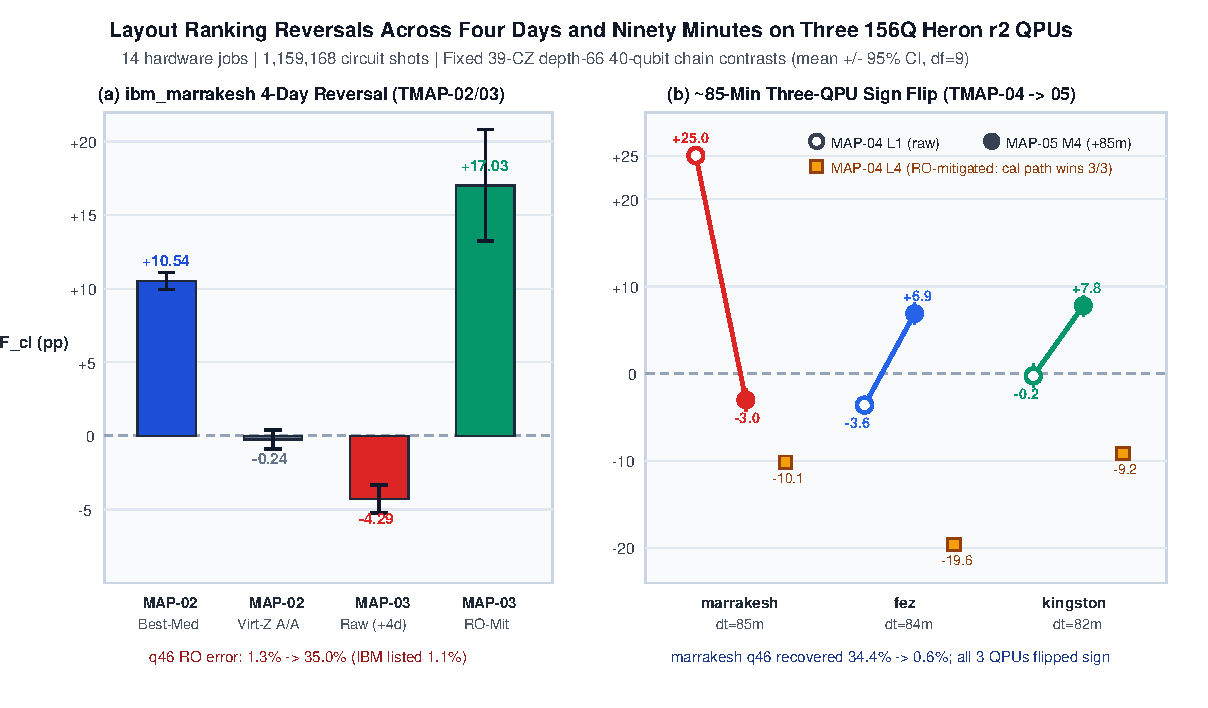
\includegraphics[width=\textwidth]{fig1_tmap_sign_reversal_three_qpus.pdf}
\caption{Layout ranking reversals across four days and eighty-five minutes on \NumBackends{} \ChipQubits{}-qubit Heron~r2 processors (\TmapSeriesJobs{} jobs, \TmapSeriesShots{} shots). (a)~On \texttt{ibm\_marrakesh}, the \TmapChainCz{}-CZ \TmapCircuitQubits{}-qubit chain contrast between the calibration-ranked best path and median path reversed from \TmapTwoPathGapPp\,pp in \texttt{TMAP-02} to \TmapThreePathGapPp\,pp \TmapThreeDaysLater{} days later in \texttt{TMAP-03} as \texttt{q46} developed a \TmapThreeQFortySixMeanPct\% assignment fault invisible to IBM's \TmapThreeQFortySixIbmPct\% snapshot; tensored readout mitigation restored a \TmapThreeMitGapPp\,pp best-path lead, while the virtual-$Z$ A/A control remained null (\TmapTwoAaVirtualZPp\,pp). (b)~Across \texttt{ibm\_marrakesh}, \texttt{ibm\_fez}, and \texttt{ibm\_kingston}, repeating the identical probe-ranked minus calibration-ranked contrast \TmapDtMinLow{}--\TmapDtMinHigh{} minutes apart (\texttt{TMAP-04} L1 open circles to \texttt{TMAP-05} M4 filled circles) reversed sign on all \NumBackends{} processors, whereas readout-mitigated contrast L4 (amber squares) favored the calibration-ranked path on every device.}\label{fig:tmap}
\end{figure*}

\begin{table*}[t]
\centering
\caption{Three-processor \TmapCircuitQubits{}-qubit chain contrasts ($\Delta F_{\mathrm{cl}}$ in percentage points across \TmapBlocks{} interleaved blocks, $\mathrm{df}=\TmapBlocksDf$, with \CiLevelPct\% confidence intervals) comparing pre-job probe-guided selection (\texttt{TMAP-04}) against exclusion and replication runs \TmapDtMinLow{}--\TmapDtMinHigh{} minutes later (\texttt{TMAP-05}). Contrast L1 and M4 measure identical probe-best minus calibration-best rules; L4 evaluates L1 after tensored readout mitigation; M1 and M2 compare $>\TmapExclThresholdPct\%$ fault exclusion against calibration-best and probe-best paths.}\label{tab:tmap_sign_reversal}
\begin{ruledtabular}
\begin{tabular}{lcclccc}
Processor & $\Delta t_{\mathrm{probe}}$ & \texttt{TMAP-04} L1: Probe$-$Cal & \texttt{TMAP-04} L4 (mit.) & \texttt{TMAP-05} M4: Probe$-$Cal & \texttt{TMAP-05} M1: Excl$-$Cal & \texttt{TMAP-05} M2: Excl$-$Probe\\
\hline
\TmapSignReversalRows
\end{tabular}
\end{ruledtabular}
\end{table*}

\subsection{Disentangling SWAP Routing from Qubit Selection (\texttt{TMAP-02})}

To isolate compilation and layout sensitivities on heavy-hex hardware without confounding circuit depth and physical qubit assignment, \texttt{TMAP-02} examined a \TmapCircuitQubits{}-qubit benchmark circuit initialized from two seed transmons rotated by $\theta=\TmapSeedThetaDeg^\circ$. In its noiseless unitary specification, the circuit concentrates output probability exclusively onto four \TmapCircuitQubits{}-bit strings,
\begin{equation}
\mathcal{S}_4 = \{0^{\TmapCircuitQubits},\, 1^{\TmapCircuitQubits},\, (10)^{\TmapStarHubDeg},\, (01)^{\TmapStarHubDeg}\},
\end{equation}
with ideal probabilities $\{\frac{1}{2}\cos^2\theta, \frac{1}{2}\cos^2\theta, \frac{1}{2}\sin^2\theta, \frac{1}{2}\sin^2\theta\}$, where each hub drives degree-\TmapStarHubDeg{} CNOT fan-out in the \emph{star} representation or an algebraically equivalent degree-2 nearest-neighbor CNOT cascade in the \emph{chain} representation. Because heavy-hex vertices have maximum degree~3, the star circuit requires extensive SABRE SWAP routing (\TmapStarFreeCz{} CZ gates unpinned in arm C1; \TmapStarOptThreeCz{} CZ at optimization level~3 and \TmapStarOptOneCz{} CZ at level~1 when pinned to a contiguous path in C2 and C3), whereas the chain embeds SWAP-free onto any simple \TmapCircuitQubits{}-qubit path in exactly \TmapChainCz{} CZ gates and depth~\TmapChainDepth{} (arms C4--C7). Primary performance is quantified by the classical Bhattacharyya fidelity $F_{\mathrm{cl}} = \sum_{x \in \mathcal{S}_4} \sqrt{p_{\mathrm{obs}}(x)\, p_{\mathrm{ideal}}(x)}$.

Scoring \TmapCandidatePaths{} candidate simple paths on \texttt{ibm\_marrakesh}'s lock-time calibration snapshot (job \texttt{\TmapTwoJobId}, \TmapTwoPubs{} PUBs, \TmapTwoShots{} shots, \TmapTwoSeconds{}\,s QPU), \texttt{TMAP-02} established four baseline results ($p_{\mathrm{Holm}} \le \TmapTwoMaxHolmP$ across all non-control contrasts; exact Wilcoxon $p_{\mathrm{Holm}} = \TmapWilcoxonFloorP$):
\begin{enumerate}
\item Eliminating SWAP routing via the star-to-chain rewrite on the \emph{identical} \TmapCircuitQubits{} transmons increased $F_{\mathrm{cl}}$ by \TmapTwoRewriteOptThreePp\,pp at optimization level~3 (\TmapStarOptThreeCz{}$\to$\TmapChainCz{} CZ) and \TmapTwoRewriteOptOnePp\,pp at level~1 (\TmapStarOptOneCz{}$\to$\TmapChainCz{} CZ), lifting raw fidelity from \TmapTwoStarFreeFcl{} (unpinned star C1) to \TmapTwoBestFcl{} (chain C5).
\item Holding gate count (\TmapChainCz{} CZ), circuit depth (\TmapChainDepth{}), and transpiler level fixed, shifting the chain from the calibration-ranked best path (C5, $F_{\mathrm{cl}}=\TmapTwoBestFcl$) to the median path (C6, $F_{\mathrm{cl}}=\TmapTwoMedFcl$) degraded fidelity by \TmapTwoPathGapPp\,pp (\CiLevelPct\% CI \TmapTwoPathGapCi)—nearly halving circuit fidelity through physical qubit selection alone [Fig.~\ref{fig:tmap}(a)].
\item The greedy calibration-scored best path outperformed Qiskit's stock level-3 layout pass (C7, $F_{\mathrm{cl}}=\TmapTwoStockFcl$) by \TmapTwoVsStockPp\,pp, inverting pre-run \texttt{FakeMarrakesh} noise-model simulations that had predicted C7 above C5 and overestimated structured-arm fidelities by roughly a factor of two.
\item Union $|0\rangle^{\otimes \TmapTwoUnionQubits}$ / $|1\rangle^{\otimes \TmapTwoUnionQubits}$ readout calibration embedded inside every block (mean error \TmapTwoUnionRoPct\%) uncovered severe undisclosed assignment faults on the losing layouts: \texttt{q42} (\TmapTwoQFortyTwoPct\%) and \texttt{q41} (\TmapTwoQFortyOnePct\%) lay on C6 and C7 while IBM's calibration snapshot reported \TmapTwoQFortyTwoIbmPct\% and \TmapTwoQFortyOneIbmPct\%.
\end{enumerate}

\subsection{Four-Day Sign Reversal from a Hidden Readout Excursion (\texttt{TMAP-03})}

To test whether the \TmapTwoPathGapPp\,pp best-versus-median path advantage represented a durable device property and to separate readout error from gate error, \texttt{TMAP-03} (preregistration \texttt{\DoiTmapThreePrereg}; job \texttt{\TmapThreeJobId}, \TmapThreePubs{} PUBs, \TmapThreeShots{} shots, \TmapThreeSeconds{}\,s QPU) replayed \texttt{TMAP-02}'s exact frozen physical layouts \TmapThreeDaysLater{} days later on \texttt{ibm\_marrakesh} alongside a $2\times 2$ structure-by-path star comparison and tensored $2\times 2$ per-qubit readout mitigation over all \TmapThreeUnionQubits{} active qubits.

Rather than replicating, the primary path contrast K1 inverted sign across all \TmapBlocks{} blocks to \TmapThreePathGapPp\,pp (\CiLevelPct\% CI \TmapThreePathGapCi, $p_{\mathrm{Holm}}=\TmapThreePathGapP$), as raw fidelity on the frozen ``best'' path dropped from \TmapTwoBestFcl{} to \TmapThreeBestFcl{} while the median path rose from \TmapTwoMedFcl{} to \TmapThreeMedFcl{} [Fig.~\ref{fig:tmap}(a)]. Simultaneously, \texttt{TMAP-02}'s losing stock layout (A3) and the day-of-execution stock layout (A4) beat the frozen best path by $\lvert\TmapThreeStockReplayGapPp\rvert$\,pp and $\lvert\TmapThreeStockTodayGapPp\rvert$\,pp, respectively, and the routed star exhibited a significant structure-by-path interaction ($\mathrm{K3}=\TmapThreeInteractionPp$\,pp, $p_{\mathrm{Holm}}=\TmapThreeInteractionP$; star gap \TmapThreeStarGapPp\,pp).

In-job union readout calibration pinpointed the physical cause: \texttt{q46}, situated on the best path (and listed at \TmapTwoQFortySixPct\% in \texttt{TMAP-02}), suffered a massive asymmetric readout excursion with $p(1|0)=\TmapThreeQFortySixZeroToOnePct\%$ and $p(0|1)=\TmapThreeQFortySixOneToZeroPct\%$ (symmetric mean error $e_{\mathrm{RO}}=\TmapThreeQFortySixMeanPct\%$), whereas IBM's execution-time calibration snapshot continued to report \texttt{q46} at \TmapThreeQFortySixIbmPct\%. Because IBM's snapshot remained blind to this fault, Qiskit's stock level-3 layout (A4) also routed through \texttt{q46}. Applying tensored inverse-assignment readout mitigation shifted the best-minus-median contrast by \TmapThreeReadoutShiftPp\,pp ($p_{\mathrm{Holm}}=\TmapThreeReadoutShiftP$), restoring a \TmapThreeMitGapPp\,pp lead for the best path ($F_{\mathrm{cl,mit}}=\TmapThreeBestMitFcl$ vs \TmapThreeMedMitFcl) and demonstrating that underlying CZ and coherence quality on the best path remained intact while single-qubit readout telegraphed.

\subsection{Three-Processor Pre-Job Probes and the Ninety-Minute Sign Flip (\texttt{TMAP-04} and \texttt{TMAP-05})}

\texttt{TMAP-03} motivated an immediate operational hypothesis: if stale readout entries corrupt layout selection, preceding each hardware benchmark with a rapid all-qubit $|0\rangle^{\otimes \ChipQubits}$ / $|1\rangle^{\otimes \ChipQubits}$ readout probe (\TmapProbePubs{} PUBs, \ProbeRepeats{} repeats per basis state, \TmapProbeSecLow{}--\TmapProbeSecHigh{}\,s QPU) and substituting $e_{\mathrm{probe}}(q)$ into the greedy path cost
\begin{equation}
\mathcal{C}(\mathcal{P}) = -\sum_{e \in \mathcal{P}} \ln\!\bigl(1 - e_{\mathrm{CZ}}(e)\bigr) - \sum_{q \in \mathcal{P}} \ln\!\bigl(1 - e_{\mathrm{RO}}(q)\bigr)
\label{eq:path_cost}
\end{equation}
should rescue path selection across processors. \texttt{TMAP-04} (preregistration \texttt{\DoiTmapFourPrereg}; \TmapFourTotalSeconds{}\,s QPU across \texttt{ibm\_marrakesh}, \texttt{ibm\_fez}, and \texttt{ibm\_kingston}) tested this rule directly, requiring a statistically significant gain ($\mathrm{L1}>0, p_{\mathrm{Holm}}<\AlphaFwer$) on at least two of \NumBackends{} processors.

As shown in Table~\ref{tab:tmap_sign_reversal}, probe-guided ranking succeeded on only \TmapFourHelpsCount{} of \NumBackends{} processors:
\begin{itemize}
\item On \texttt{ibm\_marrakesh}, \texttt{q46} remained degraded at \TmapFourQFortySixPct\% probe error (\TmapThreeQFortySixIbmPct\% listed); avoiding it raised $F_{\mathrm{cl}}$ from \TmapFourMarrCalFcl{} to \TmapFourMarrProbeFcl{} ($\mathrm{L1}=\TmapFourMarrLonePp$\,pp, \CiLevelPct\% CI \TmapFourMarrLoneCi, $p_{\mathrm{Holm}}=\TmapFourMarrLoneP$).
\item On \texttt{ibm\_fez}, where readout errors were mild and largely reflected in IBM's snapshot, probe ranking \emph{lost} to calibration ranking by $\mathrm{L1}=\TmapFourFezLonePp$\,pp (\CiLevelPct\% CI \TmapFourFezLoneCi, $p_{\mathrm{Holm}}=\TmapFourFezLoneP$).
\item On \texttt{ibm\_kingston}, although the calibration path traversed \texttt{q107} at \TmapFourKingQOneZeroSevenPct\% probe error (\TmapFourKingQOneZeroSevenIbmPct\% listed), probe and calibration paths tied ($\mathrm{L1}=\TmapFourKingLonePp$\,pp, \CiLevelPct\% CI \TmapFourKingLoneCi, $p_{\mathrm{Holm}}=\TmapFourKingLoneP$).
\end{itemize}
Crucially, after tensored readout mitigation (contrast L4), the calibration-ranked path outperformed the probe-ranked path on \emph{all \NumBackends{} processors}: \TmapFourMarrLfourMitPp\,pp on \texttt{ibm\_marrakesh}, \TmapFourFezLfourMitPp\,pp on \texttt{ibm\_fez}, and \TmapFourKingLfourMitPp\,pp on \texttt{ibm\_kingston} [amber squares in Fig.~\ref{fig:tmap}(b)]. Because Eq.~\eqref{eq:path_cost} weights one terminal readout error identically to a single CZ gate while a \TmapCircuitQubits{}-qubit chain executes \TmapChainCz{} CZ layers and cumulative idle delays, chasing small probe readout differences diverts the path onto inferior couplers and shorter-$T_2$ transmons.

To test whether surgically excluding only severely faulty transmons ($e_{\mathrm{probe}} > \TmapExclThresholdPct\%$) while preserving IBM's calibration ranking resolves this trade-off, we preregistered \texttt{TMAP-05} (\texttt{\DoiTmapFivePrereg}; \TmapFiveTotalSeconds{}\,s QPU) and executed it \TmapDtMinLow{}--\TmapDtMinHigh{} minutes after \texttt{TMAP-04} across all \NumBackends{} processors. Fault exclusion beat plain calibration ranking wherever the calibration path intersected an excluded qubit ($\mathrm{M1}=\TmapFiveFezMonePp$\,pp removing \texttt{q11} at \TmapFiveFezQElevenPct\% on \texttt{ibm\_fez}; $\mathrm{M1}=\TmapFiveKingMonePp$\,pp removing \texttt{q107} at \TmapFiveKingQOneZeroSevenPct\% on \texttt{ibm\_kingston}), while yielding a null \TmapFiveMarrMonePp\,pp on \texttt{ibm\_marrakesh} (where no excluded qubit lay on C1) and trailing full probe ranking on two devices ($\mathrm{M2}=\TmapFiveFezMtwoPp$ and \TmapFiveKingMtwoPp\,pp; Qiskit stock level~3 reached \TmapFiveFezStockFcl{} on \texttt{ibm\_fez}).

The decisive discovery of \texttt{TMAP-05}, however, emerged from contrast M4, which reran \texttt{TMAP-04}'s exact probe-versus-calibration comparison \TmapDtMinLow{}--\TmapDtMinHigh{} minutes later using identical code [Fig.~\ref{fig:tmap}(b) and Table~\ref{tab:tmap_sign_reversal}]:
\begin{align}
\texttt{ibm\_marrakesh}: &\quad \TmapFourMarrLonePp\text{\,pp} \longrightarrow \TmapFiveMarrMfourPp\text{\,pp} \quad (p_{\mathrm{Holm}}=\TmapFiveMarrMfourP), \nonumber\\
\texttt{ibm\_fez}: &\quad \TmapFourFezLonePp\text{\,pp} \longrightarrow \TmapFiveFezMfourPp\text{\,pp} \quad (p_{\mathrm{Holm}}=\TmapFiveFezMfourP), \nonumber\\
\texttt{ibm\_kingston}: &\quad \TmapFourKingLonePp\text{\,pp} \longrightarrow \TmapFiveKingMfourPp\text{\,pp} \quad (p_{\mathrm{Holm}}=\TmapFiveKingMfourP).
\end{align}
Every single processor reversed sign within ninety minutes. On \texttt{ibm\_marrakesh}, \texttt{q46} spontaneously recovered from \TmapFourQFortySixPct\% probe error at \TmapFourMarrUtc\,UTC to \TmapFiveQFortySixPct\% at \TmapFiveMarrUtc\,UTC; once \texttt{q46} healed, the calibration path no longer suffered a readout penalty and its superior gate fidelity dominated. Conversely, fresh readout excursions emerged on \texttt{ibm\_fez} and \texttt{ibm\_kingston}, flipping probe selection into a decisive win. Consequently, any single-epoch hardware comparison of qubit-selection heuristics on Heron~r2 processors measures the transient defect state of that hour rather than a time-invariant algorithmic advantage.

\section{Full-Chip Readout Time Series: Stale Snapshots, Not Crosstalk (\texttt{RO-06} and \texttt{RO-07})}\label{sec:ro}

\begin{figure*}[t]
\centering
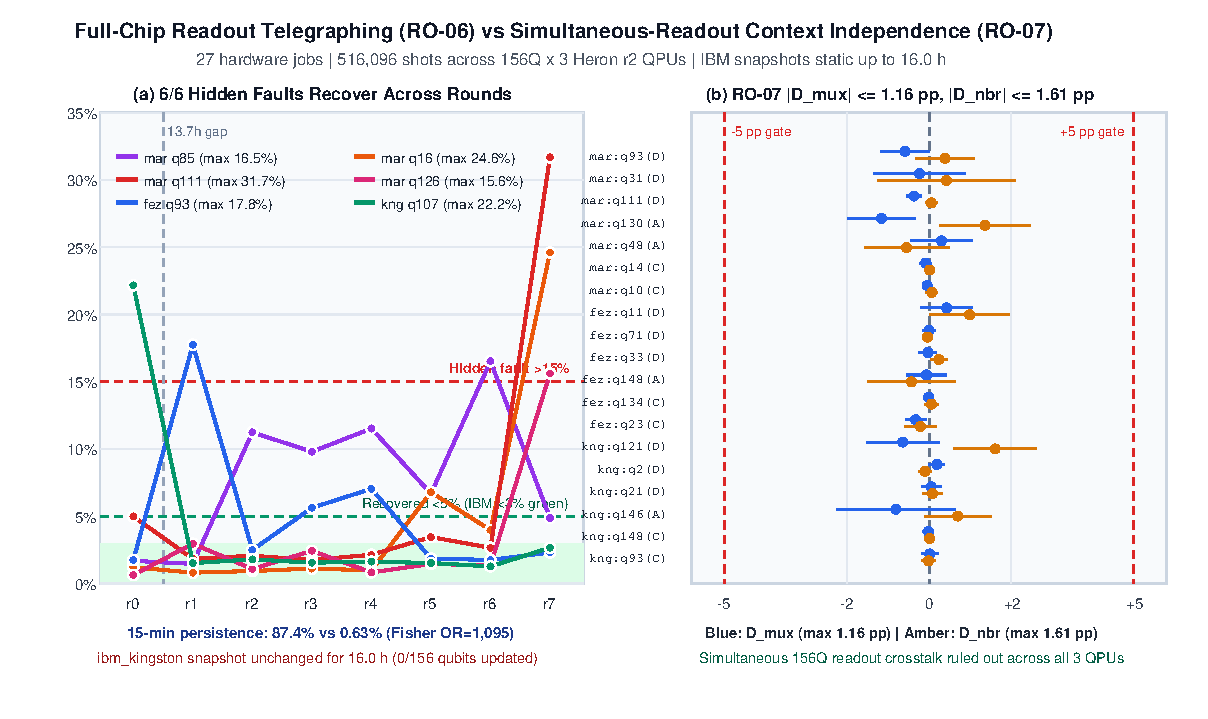
\includegraphics[width=\textwidth]{fig2_ro06_07_staleness_persistence.pdf}
\caption{Longitudinal full-chip readout telegraphing (\texttt{RO-06}) versus simultaneous-measurement context independence (\texttt{RO-07}) across \NumBackends{} \ChipQubits{}-qubit Heron~r2 processors (\RoSeriesJobs{} jobs, \RoSeriesShots{} shots). (a)~Eight-round readout trajectories for all \RoEverHidden{} transmons ever exhibiting a hidden fault ($e_{\mathrm{probe}}>\RoFaultThreshPct\%$ while $e_{\mathrm{IBM}}<\RoIbmOkThreshPct\%$, shaded green band); \RoRecoveredCount{} of \RoEverHidden{} recovered below \RoRecoveredThreshPct\% in another round, with \RoPersistFaultPct\% \RoSixIntervalMin{}-minute fault persistence (Fisher $\mathrm{OR}=\RoFisherOr$) while \texttt{ibm\_kingston}'s published snapshot remained completely static for \RoKingstonUnchangedHours{}\,h. (b)~Paired context shifts $D_{\mathrm{mux}} = e(\mathrm{ALL}) - e(\mathrm{ISO})$ (blue) and $D_{\mathrm{nbr}} = e(\mathrm{FLIP}) - e(\mathrm{ALL})$ (amber) with \CiLevelPct\% CIs across all \RoSevenTestedQubits{} target, agree, and control qubits in \texttt{RO-07}; every shift lies within $|D_{\mathrm{mux}}|\le\RoSevenMaxMuxPp$\,pp and $|D_{\mathrm{nbr}}|\le\RoSevenMaxNbrPp$\,pp, far inside the $\pm\RoContextThreshPp$\,pp preregistered crosstalk threshold.}\label{fig:ro}
\end{figure*}

\begin{table*}[t]
\centering
\caption{Summary of full-chip readout drift (\texttt{RO-06}, \RoSixJobs{} jobs across \RoSixRounds{} rounds) and simultaneous-readout context tests (\texttt{RO-07}, \RoSevenJobsCount{} jobs, \RoSevenRepeats{} interleaved repeats per condition). ``Update cadence'' lists the number of qubits (out of \ChipQubits{}) whose IBM-published \texttt{readout\_error} changed across consecutive intervals ($r_0\to r_1$ spanning \RoOvernightGapHours{}\,h, $r_1\to\dots\to r_7$ spaced by \RoSixIntervalMin{}\,min, and $r_7\to\texttt{RO-07}$ spanning \RoSevenLagMin{}\,min).}\label{tab:ro_staleness}
\begin{ruledtabular}
\begin{tabular}{llccclcc}
Processor & Hidden faults ($r_0\dots r_7$) & Mean / round & Median $\rho$ & IBM snapshot updates (\RoSixRounds{} intervals) & Max $|D_{\mathrm{mux}}|$ (pp) & Max $|D_{\mathrm{nbr}}|$ (pp)\\
\hline
\RoStalenessSummaryRows
\end{tabular}
\end{ruledtabular}
\end{table*}

Two competing physical mechanisms could explain the large discrepancies between in-job readout error $e_{\mathrm{probe}}$ and IBM's published $e_{\mathrm{IBM}}$ observed in \texttt{TMAP-02}--\texttt{TMAP-05}: (i)~\emph{measurement-context dependence}, wherein simultaneous multiplexed readout of \TmapCircuitQubits{}--\ChipQubits{} resonators or complementary neighbor excitations induces readout crosstalk absent from isolated single-qubit calibration, or (ii)~\emph{calibration snapshot staleness}, wherein transmon readout error telegraphs on hour timescales between infrequent backend calibration updates. We preregistered \texttt{RO-06} (\texttt{\DoiRoSixPrereg}) and \texttt{RO-07} (\texttt{\DoiRoSevenPrereg}) to resolve both mechanisms across all \ChipQubits{} qubits of \texttt{ibm\_marrakesh}, \texttt{ibm\_fez}, and \texttt{ibm\_kingston} (\RoSeriesJobs{} jobs, \RoSeriesShots{} shots, \RoSeriesSeconds{}\,s QPU; Table~\ref{tab:ro_staleness}).

\subsection{Prevalence, Intermittency, and Fifteen-Minute Persistence (\texttt{RO-06})}

In \texttt{RO-06}, each of \RoSixRounds{} rounds submitted synchronized full-chip $|0\rangle^{\otimes \ChipQubits}$ and $|1\rangle^{\otimes \ChipQubits}$ probe jobs (\ProbeRepeats{} repeats per state, \ShotsPerPub{} shots) to all \NumBackends{} processors while recording each backend's live calibration snapshot. Following client sleep after round~0 (\RoOvernightGapHours{}\,h overnight interval), rounds~1--7 sampled continuously every \RoSixIntervalMin{}\,min over \RoActiveSpanHours{}\,h. Defining a \emph{hidden fault} prospectively as $e_{\mathrm{probe}}(q) > \RoFaultThreshPct\%$ concurrent with $e_{\mathrm{IBM}}(q) < \RoIbmOkThreshPct\%$, and \emph{recovery} as $e_{\mathrm{probe}}(q) < \RoRecoveredThreshPct\%$, the four preregistered hypotheses yielded:
\begin{enumerate}
\item \emph{Rarity (H1 not supported):} Hidden faults averaged \RoMinHiddenMean{}--\RoMaxHiddenMean{} qubits per processor-round (Table~\ref{tab:ro_staleness}), appearing in fewer than half of rounds on every device. Chronically degraded readout channels exist on each chip, but most are accurately flagged by IBM's calibration (median probe-versus-IBM Spearman rank correlation $\rho = \RoRhoMarr$, \RoRhoFez, and \RoRhoKing{} on \texttt{ibm\_marrakesh}, \texttt{ibm\_fez}, and \texttt{ibm\_kingston}).
\item \emph{Complete intermittency (H2 supported):} Every single one (\RoRecoveredCount{} of \RoEverHidden{}) of the transmons that crossed the hidden-fault threshold in at least one round recovered below \RoRecoveredThreshPct\% in another round [Fig.~\ref{fig:ro}(a)]. Additional rapid recoveries occurred during the \RoSevenLagMin{}-minute window between \texttt{RO-06} round~7 and \texttt{RO-07}, where \RoSevenDisagreeRecovered{} of \RoSevenDisagreeTotal{} targeted discrepancy qubits healed below \RoRecoveredThreshPct\% (including \texttt{ibm\_marrakesh} \texttt{q111} dropping from \RoSevenMarrQOneElevenPrePct\% to \RoSevenMarrQOneElevenPostPct\%).
\item \emph{Tens-of-minutes persistence (H3 supported):} Pooling consecutive round transitions across all $\NumBackends{} \times \ChipQubits{}$ device-qubits yielded transition counts $(\text{ok}\to\text{ok}, \text{ok}\to\text{fault}, \text{fault}\to\text{ok}, \text{fault}\to\text{fault}) = (\RoTransitionOkOk, \RoTransitionOkFault, \RoTransitionFaultOk, \RoTransitionFaultFault)$. A transmon faulty ($>\RoFaultThreshPct\%$) in round~$r$ remained faulty in round~$r+1$ with probability \RoPersistFaultPct{}, compared to \RoPersistOkPct{} for a healthy qubit (Fisher exact odds ratio $\mathrm{OR}=\RoFisherOr$, $p=\RoFisherP$). Restricting strictly to the \RoSixIntervalMin{}-minute pairs $r_1\to\dots\to r_7$ strengthened persistence to \RoSensPersistFaultPct\% versus \RoSensPersistOkPct\% ($\mathrm{OR}=\RoSensFisherOr$, $p=\RoSensFisherP$). Within-round repeat spread had a median range of \RoWithinSpreadPp\,pp versus \RoBetweenChangePp\,pp between rounds on flagged qubits, confirming genuine physical state transitions rather than binomial shot noise.
\end{enumerate}

\subsection{Eliminating Simultaneous-Readout Crosstalk (\texttt{RO-07}) and Measuring Snapshot Cadence}

\texttt{RO-07} directly tested whether full-chip simultaneous measurement inflates $e_{\mathrm{probe}}$ relative to isolated single-qubit readout. Using a deterministic rule applied to \texttt{RO-06} round~7, \RoSevenTestedQubits{} mutually uncoupled transmons across the \NumBackends{} processors (\RoSevenDisagreeTotal{} \texttt{DISAGREE} qubits with largest $e_{\mathrm{probe}} - e_{\mathrm{IBM}}$, plus \texttt{AGREE} high-error and clean \texttt{CONTROL} qubits) were measured across \RoSevenRepeats{} interleaved repeats of three contexts: isolated readout of only the selected subset (\texttt{ISO}), simultaneous readout of all \ChipQubits{} qubits prepared identically (\texttt{ALL}), and simultaneous readout with all non-target qubits inverted into the complementary state $1-b$ (\texttt{FLIP}).

Both context-crosstalk hypotheses failed decisively [Fig.~\ref{fig:ro}(b) and Table~\ref{tab:ro_staleness}]. Across all \RoSevenTestedQubits{} tested qubits on all \NumBackends{} processors, the multiplexing shift $|D_{\mathrm{mux}}| = |e(\mathrm{ALL}) - e(\mathrm{ISO})|$ never exceeded \RoSevenMaxMuxPp\,pp, the neighbor state-flip shift $|D_{\mathrm{nbr}}| = |e(\mathrm{FLIP}) - e(\mathrm{ALL})|$ never exceeded \RoSevenMaxNbrPp\,pp, and clean control qubits varied by at most \RoSevenControlsMaxPp\,pp—nearly an order of magnitude below the preregistered \RoContextThreshPp\,pp threshold required to explain \RoFaultThreshPct\%--\TmapThreeQFortySixZeroToOnePct\% hidden faults.

Inspecting the discrete update cadence of IBM's calibration snapshots across all nine timestamps (\texttt{RO-06} rounds~0--7 plus \texttt{RO-07}) resolved the discrepancy completely (Table~\ref{tab:ro_staleness}). During the continuous \RoActiveSpanHours{}\,h daytime window of \RoSixIntervalMin{}-minute sampling, \emph{zero} qubits updated on any of the \NumBackends{} processors; on \texttt{ibm\_kingston}, zero of \ChipQubits{} readout error entries changed across the entire \RoKingstonUnchangedHours{}\,h span. Moreover, when \texttt{ibm\_fez}'s calibration table refreshed between round~7 and \texttt{RO-07} (updating \RoFezUpdatedQubits{} of \ChipQubits{} qubits), Spearman rank agreement between IBM's newly published readout errors and our immediately preceding round~6 and round~7 full-chip probes jumped to $\rho = \RoFezNewRhoRoundSix$ and \RoFezNewRhoRoundSeven{} (median absolute gap \RoFezNewGapRoundSevenPp\,pp), compared with $\rho = \RoFezOldRho$ (gap \RoFezOldGapPp\,pp) for the stale snapshot they replaced. Thus, provider readout calibrations and full-chip user probes measure the same physical quantity; hidden faults arise because transmon readout telegraphs on hour timescales inside multi-hour calibration blind spots.

\section{Spatially Separated Couplers and Why White-Noise Nulls Misclassify Local $1/f$ Drift (\texttt{CN-01})}\label{sec:cn01}

\begin{figure*}[t]
\centering
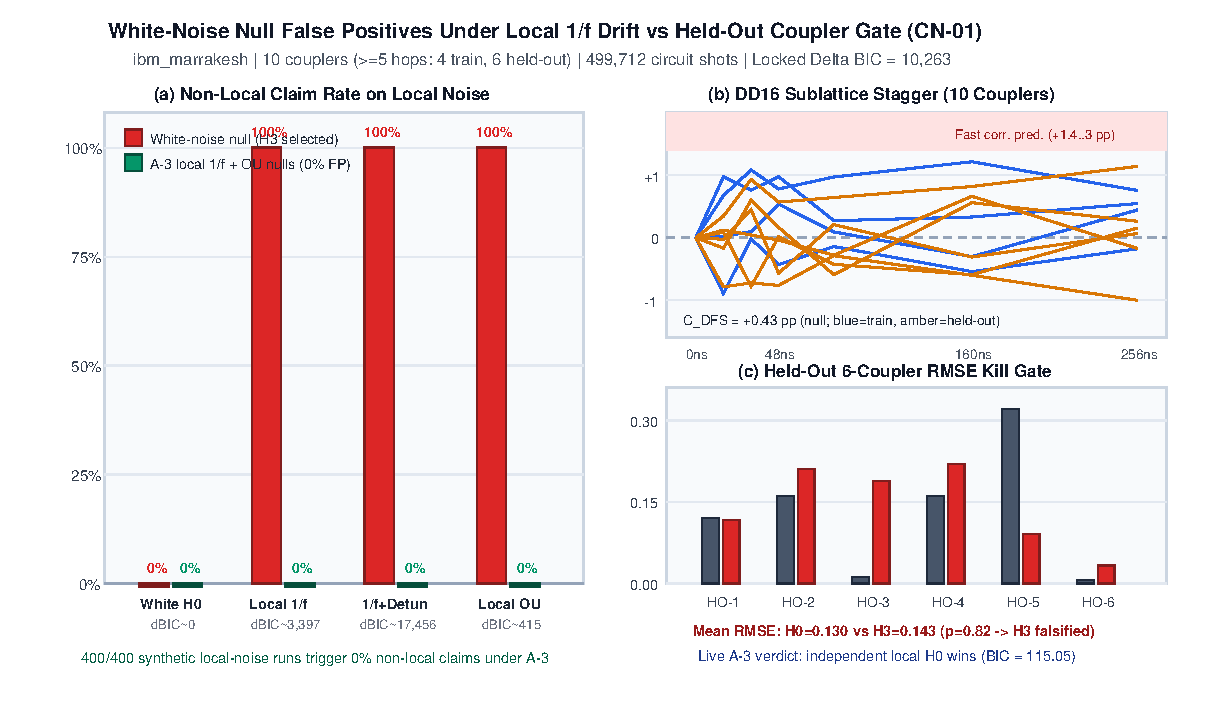
\includegraphics[width=\textwidth]{fig3_cn01_colored_noise_heldout_gate.pdf}
\caption{Diagnosing white-noise null misspecification and bounding non-local dephasing across \CnTotalCouplers{} spatially separated couplers on \texttt{ibm\_marrakesh} (\texttt{CN-01}, job \texttt{\CnJobId}, \CnPubs{} PUBs, \CnShots{} circuit shots). (a)~Pre-execution validation across \CnValTotalReps{} synthetic datasets (\CnValLocalNullReps{} purely local-noise truths): under a white-noise-only null ($H_0$), generalized least squares falsely selects the spatially correlated non-Markovian bath $H_3$ in \CnValOneFHThreePct\% of local $1/f$, detuned $1/f$, and local OU runs with median $\Delta\mathrm{BIC}$ up to \CnValDetunedMedDbic, whereas adding local colored-noise nulls (amendment A-3) reduces false non-local claims to \CnValAThreeLocalFpPct\%. (b)~Measured DD16 $\Phi^+$ Bell fidelity shifts across sublattice stagger offsets $\Delta \in [0, \CnMaxStaggerNs]$\,ns for all \CnTotalCouplers{} couplers ($\ge\CnMinHops$ hops apart), showing flat profiles ($C_{\mathrm{DFS}}=\CnCdfsMeanPp$\,pp) well below the fast correlated-dephasing band. (c)~On the \CnHeldOutCouplers{} spatially held-out couplers, $H_3$ fails to improve prediction RMSE over $H_0$ (\CnHoRmseHThree{} vs \CnHoRmseHZero, $p=\CnHoPVal$), triggering its preregistered kill gate in agreement with A-3 ($\mathrm{BIC}_{H_0}=\CnAThreeBicHZero$).}\label{fig:cn01}
\end{figure*}

\begin{table*}[t]
\centering
\caption{Summary of \texttt{CN-01} across \CnTotalCouplers{} couplers ($\ge\CnMinHops$ heavy-hex hops apart; \CnTrainCouplers{} training, \CnHeldOutCouplers{} held-out) on \texttt{ibm\_marrakesh}. Top: mechanistic contrasts across all \CnTotalCouplers{} couplers ($\mathrm{df}=\TmapBlocksDf$, Holm-adjusted). Middle: training-cohort GLS selection comparing the locked \CnLockedConds{}-condition white-noise-null specification against the \CnAThreeConds{}-condition A-3 colored-null specification. Bottom: \CnValTotalReps{}-replicate synthetic validation rates prior to hardware analysis.}\label{tab:cn01_heldout_nulls}
\begin{ruledtabular}
\begin{tabular}{llrrrrr}
\multicolumn{7}{l}{\textbf{(a) Hardware mechanistic contrasts across \CnTotalCouplers{} couplers ($\mathrm{df}=\TmapBlocksDf$, Holm-corrected)}}\\
Contrast & \multicolumn{3}{l}{Physical observable} & Mean (pp) & \CiLevelPct\% CI (pp) & Holm $p$\\
\hline
\CnContrastRows
\hline
\multicolumn{7}{l}{\textbf{(b) Training-cohort GLS fits (\CnTrainCouplers{} couplers; held-out RMSE $H_0=\CnHoRmseHZero$ vs $H_3=\CnHoRmseHThree$, $t_{\CnHeldOutDf}=\CnHoTStat$, $p=\CnHoPVal$)}}\\
Noise hypothesis & Scope & $k$ & $\chi^2_{\mathrm{lock}}$ & $\mathrm{BIC}_{\mathrm{lock}}$ & $\chi^2_{\mathrm{A3}}$ & $\mathrm{BIC}_{\mathrm{A3}}$\\
\hline
\CnModelBicRows
\hline
\multicolumn{7}{l}{\textbf{(c) Pre-execution synthetic validation (\CnValTotalReps{} replicates across seven ground-truth baths)}}\\
Synthetic ground truth & Replicates & Med.\ $\Delta\mathrm{BIC}_{\mathrm{lock}}$ & Lock $H_3$ sel. & Lock Stage-2 & A-3 non-local & A-3 corr.\ deph.\\
\hline
\CnValidationRows
\end{tabular}
\end{ruledtabular}
\end{table*}

Whereas Sections~\ref{sec:tmap} and~\ref{sec:ro} establish how temporal drift in single-qubit readout corrupts spatial compilation rankings, \texttt{CN-01} (\texttt{\DoiCnZeroOne}; job \texttt{\CnJobId}, \CnPubs{} PUBs, \CnShots{} circuit shots, \CnCouplerShots{} multiplexed coupler-shots, \CnSeconds{}\,s QPU on \texttt{ibm\_marrakesh}) addresses the complementary inference hazard: how ordinary local low-frequency dephasing masquerades as spatially correlated non-Markovian memory when benchmarked against a white-noise null.

\subsection{Sublattice Toggling-Frame Spectroscopy Across Ten Distant Couplers}

Ten two-qubit couplers at pairwise graph distance $\ge\CnMinHops$ heavy-hex hops were measured simultaneously inside every circuit across three Pauli tomography bases. Under $N$-pulse periodic dynamical decoupling over total window $T = \CnDdWindowUs\,\mu\text{s}$ ($N=\CnDdSixteenPulses$ slot width $\tau_{\mathrm{slot}} = \CnSlotNs$\,ns), shifting the $\pi$-pulse train on one heavy-hex sublattice relative to its partner by temporal stagger $\Delta \in [0, \CnMaxStaggerNs]$\,ns continuously tunes their toggling-frame sign overlap~\cite{pazsilva2017,tripathi2022}:
\begin{equation}
\alpha_{uv}(\Delta) = 1 - \frac{2\Delta}{\tau_{\mathrm{slot}}}.
\label{eq:toggling_overlap}
\end{equation}
For Markovian or fast-correlating cross-dephasing $\gamma_{uv}$ shared across a coupler's two transmons $(u, v)$, the Bell-state coherence decay rates split oppositely between the correlated ($\Phi^\pm$) and anti-correlated ($\Psi^\pm$) parity subspaces:
\begin{equation}
\Gamma_{\Phi^\pm}(\Delta) = \gamma_u + \gamma_v + 2\alpha_{uv}(\Delta)\gamma_{uv}, \qquad
\Gamma_{\Psi^\pm}(\Delta) = \gamma_u + \gamma_v - 2\alpha_{uv}(\Delta)\gamma_{uv}.
\label{eq:dfs_rates}
\end{equation}
Increasing $\Delta$ from $0$ to $\CnMaxStaggerNs$\,ns drives $\alpha_{uv}$ from $+1$ to $0$, enhancing $\Phi^+$ Bell fidelity while symmetrically depressing $\Psi^+$ fidelity ($C_{\mathrm{DFS}} > 0$). Purely local dephasing ($\gamma_{uv}=0$) affects both subspaces identically; static spectator $ZZ$ coupling appears only when an adjacent spectator is prepared in $|{+}\rangle$ ($C_{\mathrm{spec}} > 0$); and finite-duration drive-envelope collisions produce a sharp step completed by $\Delta = \CnCollisionStepNs$\,ns ($S_{48} \ge \CnStepGate$).

On live hardware, all four preregistered mechanistic contrasts across the \CnTotalCouplers{} couplers were statistically indistinguishable from zero [Table~\ref{tab:cn01_heldout_nulls}(a) and Fig.~\ref{fig:cn01}(b)]: $C_{\mathrm{DFS}} = \CnCdfsMeanPp$\,pp (\CiLevelPct\% CI \CnCdfsCi, $p_{\mathrm{Holm}}=\CnCdfsP$), $C_{\mathrm{spec}} = \CnCspecMeanPp$\,pp ($p_{\mathrm{Holm}}=\CnCspecP$), $C_{\mathrm{stag}} = \CnCstagMeanPp$\,pp ($p_{\mathrm{Holm}}=\CnCstagP$), and pulse-number memory contrast $C_{\mathrm{mem}} = \CnCmemMeanPp$\,pp ($p_{\mathrm{Holm}}=\CnCmemP$), with step fraction $S_{48} = \CnStepFractionS$ and A/A sentinel RMS drift \CnAaRmsRawPp\,pp. Fast spatially correlated dephasing on timescales shorter than the \CnSlotNs{}\,ns DD slot is bounded below \CnFastBoundPp\,pp.

\subsection{In-Sample $\Delta\mathrm{BIC}$ Inflation Versus Held-Out Spatial Falsification}

Despite all mechanistic signatures being null, fitting the originally locked \CnLockedConds{}-condition generalized least-squares (GLS) hierarchy on the \CnTrainCouplers{} training couplers selected the \CnBicGate{}-parameter non-local Ornstein--Uhlenbeck bath hypothesis ($H_3$) over the local white-noise null ($H_0$) by an overwhelming $\Delta\mathrm{BIC} = \CnLockedDeltaBic$ ($\mathrm{BIC}_{H_3} = \CnLockedBicHThree$ vs $\mathrm{BIC}_{H_0} = \CnLockedBicHZero$, well above the $\Delta\mathrm{BIC}\ge\CnBicGate$ selection gate). Without out-of-sample protection, such an information-criterion gap would routinely be misreported as strong evidence for non-Markovian correlated bath memory.

Here, the preregistered spatial kill criterion intervened decisively [Fig.~\ref{fig:cn01}(c)]: when evaluated on the \CnHeldOutCouplers{} spatially disjoint held-out couplers measured in the exact same shots, $H_3$ yielded a worse prediction error ($\mathrm{RMSE}_{H_3} = \CnHoRmseHThree$) than the parameter-free white-noise baseline ($\mathrm{RMSE}_{H_0} = \CnHoRmseHZero$; paired $t_{\CnHeldOutDf} = \CnHoTStat$, two-sided $p = \CnHoPVal$), falsifying the transferable memory claim and halting Stage-2 replication.

To understand why in-sample white-noise GLS produced $\Delta\mathrm{BIC} = \CnLockedDeltaBic$ on a null dataset, \CnValTotalReps{} synthetic datasets were generated in the locked bit layout using empirical $T_1$, readout error, and block drift [Table~\ref{tab:cn01_heldout_nulls}(c) and Fig.~\ref{fig:cn01}(a)]. Whenever the synthetic ground truth contained \emph{purely independent local} $1/f$ dephasing, local $1/f$ with small Ramsey frame detuning, or local OU noise, the white-noise-null specification falsely selected non-local $H_3$ in \CnValOneFHThreePct\% of replicates with median $\Delta\mathrm{BIC}$ of \CnValOneFMedDbic, \CnValDetunedMedDbic, and \CnValOuMedDbic, respectively—and even bypassed the held-out gate in \CnValLocalStageTwoLowPct\%--\CnValLocalStageTwoHighPct\% of replicates because $H_0$ and $H_3$ were calibrated from mismatched free-induction versus echo baselines. On hardware, single-quadrature Ramsey fidelity decayed to \CnRamseySixteenMean{} at $\CnLongWindowUs\,\mu\text{s}$ compared with \CnEchoSixteenMean{} under Hahn echo and \CnDdThirtyTwoSixteenMean{} under \CnDdThirtyTwoPulses{}-pulse DD—ordinary local low-frequency dephasing and frame detuning that $H_0$ cannot absorb.

Incorporating local colored-noise nulls ($H_{0,1/f}$ and local uncorrelated OU $H_{3,\mathrm{loc}}$), removing single-quadrature Ramsey arms from the multi-model fit (\CnAThreeConds{} conditions), calibrating all hypotheses from a common echo-DD32 reference, and hash-seeding the training split (amendment A-3, SHA-256 \texttt{\CnAmendShaPrefix\ldots}, recorded locally prior to job submission and reported alongside the locked pipeline for full transparency) eliminated non-local false positives across all \CnValLocalNullReps{} synthetic local-noise replicates (\CnValAThreeLocalFpPct\% false-claim rate; \CnValAThreeFastPowPct\%--\CnValAThreeMarkovPowPct\% power on fast correlated truths). Applied to the live \texttt{CN-01} counts, A-3 selected independent local $H_0$ ($\mathrm{BIC} = \CnAThreeBicHZero$, beating $H_1$ at \CnAThreeBicHOne{} by \CnAThreeRunnerUpGap{} BIC units; refitting with an unconstrained white-noise floor above \CnWhiteFloorCapKhz\,kHz collapsed $H_{0,1/f}$, $H_{3,\mathrm{loc}}$, and $H_3$ identically onto $H_0$ at \CnSolvedWhiteFloorKhz\,kHz), bringing in-sample selection into full agreement with both the mechanistic contrasts and the held-out spatial gate.

\section{Design Rules for Reproducible NISQ Benchmarking}\label{sec:rules}

Synthesizing all \TotalJobs{} hardware jobs across \texttt{ibm\_marrakesh}, \texttt{ibm\_fez}, and \texttt{ibm\_kingston} yields four actionable experimental design rules for superconducting processor benchmarking, compiler evaluation, and noise spectroscopy:

\begin{enumerate}
\item \textbf{Mandatory Interleaved Block Randomization and Embedded A/A Sentinels.} Because transmon readout and coherent gain drift measurably over minutes, circuit arms must never be submitted sequentially or analyzed with shot-level binomial error bars. Interleaving randomized blocks with identical-circuit A/A sentinels empirically anchors the within-job drift floor (\TmapTwoAaVirtualZPp\,pp virtual-$Z$ A/A contrast in \texttt{TMAP-02}; \CnAaRmsRawPp\,pp RMS sentinel floor in \texttt{CN-01}) and turns block means into valid paired replicates.
\item \textbf{Pre-Job Surgical Readout Screening Rather Than Blind Calibration or Probe Re-Weighting.} Provider readout calibrations on \ChipQubits{}-qubit Heron~r2 processors are accurate immediately after refresh ($\rho \approx \RoFezNewRhoRoundSeven$) yet remain static for up to \RoKingstonUnchangedHours{}\,h while individual qubits telegraph above \RoFaultThreshPct\%--\TmapThreeQFortySixZeroToOnePct\% for tens of minutes (\RoPersistFaultPct\% \RoSixIntervalMin{}-minute persistence). Replacing published readout weights globally with a pre-job probe degrades gate and coherence selection once readout is mitigated (\texttt{TMAP-04} L4 negative on all \NumBackends{} QPUs). Instead, practitioners should run a rapid \TmapProbePubs{}-PUB all-qubit $|0\rangle$/$|1\rangle$ probe immediately before execution, mask out only transmons exceeding a gross fault ceiling ($e_{\mathrm{probe}} > \TmapExclThresholdPct\%$), and embed two union $|0\rangle$/$|1\rangle$ circuits per block to audit in-job stability.
\item \textbf{Multi-Epoch Replication Across Calibration Windows for Compiler Claims.} Because probe-versus-calibration rankings inverted sign across all \NumBackends{} processors within \TmapDtMinLow{}--\TmapDtMinHigh{} minutes (\texttt{TMAP-04}$\to$\texttt{TMAP-05}) and across \TmapThreeDaysLater{} days (\texttt{TMAP-02}$\to$\texttt{TMAP-03}), single-job layout or routing benchmarks characterize a transient defect realization rather than an intrinsic compiler advantage. Algorithmic routing claims require replication across separated hours and calibration epochs.
\item \textbf{Local Colored-Noise Nulls Paired with Spatially Held-Out Generalization Gates.} In bath-correlation or non-Markovian spectroscopy, white-noise-only nulls guarantee spurious in-sample discovery ($\Delta\mathrm{BIC}$ reaching \CnValOuMedDbic{}--\CnValDetunedMedDbic) whenever ordinary local $1/f$ or telegraph dephasing is present. Preregistrations must include local $1/f$ and local Ornstein--Uhlenbeck nulls, calibrate competing hypotheses on matched pulse-echo baselines rather than phase-sensitive Ramsey decays, verify a \CnValAThreeLocalFpPct\% false-positive rate on synthetic local-colored-noise simulations prior to hardware spend, and enforce out-of-sample RMSE improvement on spatially disjoint couplers measured simultaneously in the same shots.
\end{enumerate}

\section{Data and Code Availability}\label{sec:data}

All raw \texttt{SamplerV2} bitstring count histograms (\TotalPubs{} PUBs, \TotalShots{} circuit shots across \TotalJobs{} verified hardware jobs), compiled \texttt{.qpy} circuit binaries, pre-submission SHA-256 lock manifests, submission receipts, backend calibration snapshots, and analysis scripts are permanently archived across \NumZenodoLetters{} Zenodo data records and \NumZenodoPreregs{} prospective Zenodo preregistrations:
\begin{itemize}
\item \textbf{\texttt{TMAP-02}:} Data and code at \texttt{\DoiTmapTwo}~\cite{davis_tmap02}.
\item \textbf{\texttt{TMAP-03}:} Preregistration at \texttt{\DoiTmapThreePrereg}~\cite{prereg_tmap03}; data and code at \texttt{\DoiTmapThree}~\cite{davis_tmap03}.
\item \textbf{\texttt{TMAP-04}:} Preregistration at \texttt{\DoiTmapFourPrereg}~\cite{prereg_tmap04}; data and code at \texttt{\DoiTmapFour}~\cite{davis_tmap04}.
\item \textbf{\texttt{TMAP-05}:} Preregistration at \texttt{\DoiTmapFivePrereg}~\cite{prereg_tmap05}; data and code at \texttt{\DoiTmapFive}~\cite{davis_tmap05}.
\item \textbf{\texttt{RO-06} and \texttt{RO-07}:} Preregistrations at \texttt{\DoiRoSixPrereg}~\cite{prereg_ro06} and \texttt{\DoiRoSevenPrereg}~\cite{prereg_ro07}; combined longitudinal and context data at \texttt{\DoiRoSixSeven}~\cite{davis_ro0607}.
\item \textbf{\texttt{CN-01}:} Stage-1 data, A-3 validation suite, and diagnostic records at \texttt{\DoiCnZeroOne}~\cite{davis_cn01}.
\end{itemize}
Accompanying this unified manuscript in \texttt{papers/heron\_r2\_calibration\_staleness\_and\_colored\_nulls/} are \texttt{generate\_unified\_assets.py}, \texttt{generated.tex}, the vector figures, \texttt{SHA256SUMS.txt}, and \texttt{reproducibility\_capsule.json} (\texttt{schema: "osiris.reproducibility\_capsule/1"}, RFC~8785 canonical SHA-256 prefix \texttt{\CapsuleRfcShaPrefix\ldots}, binding all \TotalJobs{} IBM Quantum \texttt{job\_id}s and \CapsuleSourceCount{} source JSON SHA-256 digests).

\begin{acknowledgments}
We acknowledge the use of IBM Quantum services for this work; the views expressed are those of the author and do not reflect the official policy or position of IBM or the IBM Quantum team. Experiment-automation software, deterministic asset generation, and manuscript preparation were carried out with the assistance of AI coding tools under the author's direction, cryptographic pre-submission locking, and verification.
\end{acknowledgments}

\begin{thebibliography}{99}

\bibitem{klimov2018}
P.~V.~Klimov \emph{et al.}, Fluctuations of energy-relaxation times in superconducting qubits, Phys.\ Rev.\ Lett.\ \textbf{121}, 090502 (2018).

\bibitem{burnett2019}
J.~J.~Burnett \emph{et al.}, Decoherence benchmarking of superconducting qubits, npj Quantum Inf.\ \textbf{5}, 54 (2019).

\bibitem{proctor2020}
T.~Proctor, M.~Revelle, E.~Nielsen, K.~Rudinger, D.~Lobser, P.~Maunz, R.~Blume-Kohout, and K.~Young, Detecting and tracking drift in quantum information processors, Nat.\ Commun.\ \textbf{11}, 5396 (2020).

\bibitem{thorbeck2023}
T.~Thorbeck, A.~Eddins, I.~Lauer, D.~T.~McClure, and M.~Carroll, Two-level-system dynamics in a superconducting qubit due to background ionizing radiation, PRX Quantum \textbf{4}, 020356 (2023).

\bibitem{nation2023}
P.~D.~Nation and M.~Treinish, Suppressing quantum circuit errors due to system variability, PRX Quantum \textbf{4}, 010327 (2023).

\bibitem{pazsilva2017}
G.~A.~Paz-Silva, L.~M.~Norris, and L.~Viola, Multiqubit spectroscopy of Gaussian quantum noise, Phys.\ Rev.\ A \textbf{95}, 022121 (2017).

\bibitem{sung2021}
Y.~Sung \emph{et al.}, Multi-level quantum noise spectroscopy, Nat.\ Commun.\ \textbf{12}, 967 (2021).

\bibitem{tripathi2022}
V.~Tripathi, H.~Chen, M.~Khezri, K.-W.~Yip, E.~M.~Levenson-Falk, and D.~A.~Lidar, Suppression of crosstalk in superconducting qubits using dynamical decoupling, Phys.\ Rev.\ Applied \textbf{18}, 024068 (2022).

\bibitem{chamberland2020}
C.~Chamberland, G.~Zhu, T.~J.~Yoder, J.~B.~Hertzberg, and A.~W.~Cross, Topological and subsystem codes on low-degree graphs with flag qubits, Phys.\ Rev.\ X \textbf{10}, 011022 (2020).

\bibitem{chen2023}
E.~H.~Chen \emph{et al.}, Detector tomography on IBM quantum computers and mitigation of an imperfect measurement, Phys.\ Rev.\ A \textbf{107}, 032602 (2023).

\bibitem{cywinski2008}
{\L}.~Cywi{\'n}ski, R.~M.~Lutchyn, C.~P.~Nave, and S.~Das~Sarma, How to enhance dephasing time in superconducting qubits, Phys.\ Rev.\ B \textbf{77}, 174509 (2008).

\bibitem{bylander2011}
J.~Bylander \emph{et al.}, Noise spectroscopy through dynamical decoupling with a superconducting flux qubit, Nat.\ Phys.\ \textbf{7}, 565 (2011).

\bibitem{davis_tmap02}
D.~P.~Davis, Same gate count, half the fidelity: a preregistered decomposition of layout, routing and optimisation-level effects on a 40-qubit circuit on \texttt{ibm\_marrakesh}, Zenodo (2026), \texttt{doi:\DoiTmapTwo}.

\bibitem{davis_cn01}
D.~P.~Davis, No evidence of spatially correlated or non-Markovian dephasing across ten couplers of \texttt{ibm\_marrakesh} --- and why a white-noise null is not enough to look for it, Zenodo (2026), \texttt{doi:\DoiCnZeroOne}.

\bibitem{prereg_tmap03}
D.~P.~Davis, Preregistration: layout replication and readout attribution on \texttt{ibm\_marrakesh} (\texttt{TMAP-03}), Zenodo (2026), \texttt{doi:\DoiTmapThreePrereg}.

\bibitem{davis_tmap03}
D.~P.~Davis, Four days later, the best qubits were the worst: a preregistered replication on \texttt{ibm\_marrakesh} in which readout faults invisible to the published calibration reversed a 10\,pp layout effect, Zenodo (2026), \texttt{doi:\DoiTmapThree}.

\bibitem{prereg_tmap04}
D.~P.~Davis, Preregistration: three-processor probe-guided qubit selection (\texttt{TMAP-04}), Zenodo (2026), \texttt{doi:\DoiTmapFourPrereg}.

\bibitem{davis_tmap04}
D.~P.~Davis, A per-job readout probe rescues qubit selection on one IBM Heron~r2 processor and hurts it on another: a preregistered three-device test, Zenodo (2026), \texttt{doi:\DoiTmapFour}.

\bibitem{prereg_tmap05}
D.~P.~Davis, Preregistration: probe-threshold fault exclusion across three Heron~r2 processors (\texttt{TMAP-05}), Zenodo (2026), \texttt{doi:\DoiTmapFivePrereg}.

\bibitem{davis_tmap05}
D.~P.~Davis, Qubit-selection rules for IBM Heron~r2 do not hold their ranking for ninety minutes: a preregistered exclusion test and an unplanned sign flip on three processors, Zenodo (2026), \texttt{doi:\DoiTmapFive}.

\bibitem{prereg_ro06}
D.~P.~Davis, Preregistration: full-chip longitudinal readout fault persistence across three Heron~r2 processors (\texttt{RO-06}), Zenodo (2026), \texttt{doi:\DoiRoSixPrereg}.

\bibitem{prereg_ro07}
D.~P.~Davis, Preregistration: isolated versus simultaneous full-chip readout context test (\texttt{RO-07}), Zenodo (2026), \texttt{doi:\DoiRoSevenPrereg}.

\bibitem{davis_ro0607}
D.~P.~Davis, Stale snapshots, not hidden physics: readout faults on three IBM Heron~r2 processors are rare, persist for tens of minutes, and do not depend on measurement context, Zenodo (2026), \texttt{doi:\DoiRoSixSeven}.

\end{thebibliography}

\end{document}
